%\documentclass[10pt,twocolumn,letterpaper,draft]{article}
\documentclass[10pt,letterpaper]{ctexart}

\usepackage{cvpr}
\usepackage{graphicx}
\usepackage{wrapfig}
\usepackage{amsmath}
\newtheorem{myDef}{Definition}
\newtheorem{myTheo}{Theorem}

\usepackage{amssymb}
% \usepackage{color}
\usepackage{subfigure}
\usepackage{algorithm}
\usepackage{algorithmicx}
\usepackage{algpseudocode}
\usepackage{pythonhighlight}
\usepackage{xcolor}
\usepackage{listings}
\lstset{language=C++,
    basicstyle=\ttfamily,
    frame=single,
    keywordstyle=\color{blue}\ttfamily,
    stringstyle=\color{magenta}\ttfamily,
    commentstyle=\color{green}\ttfamily,
    morecomment=[l][\color{magenta}]{\#},
    morekeywords={*,uint_fast64_t}
}

\renewcommand{\labelenumi}{\alph{enumi}.} % Make numbering in the enumerate environment by letter rather than number (e.g. section 6)
\floatname{algorithm}{算法}
\renewcommand{\algorithmicrequire}{\textbf{输入:}}
\renewcommand{\algorithmicensure}{\textbf{输出:}}
\renewcommand{\lstlistingname}{代码清单}

\usepackage{enumitem}
\setenumerate[1]{itemsep=0pt,partopsep=0pt,parsep=\parskip,topsep=5pt}
\setitemize[1]{itemsep=0pt,partopsep=0pt,parsep=\parskip,topsep=5pt}
\setdescription{itemsep=0pt,partopsep=0pt,parsep=\parskip,topsep=5pt}

% Include other packages here, before hyperref.

% If you comment hyperref and then uncomment it, you should delete
% egpaper.aux before re-running latex.  (Or just hit 'q' on the first latex
% run, let it finish, and you should be clear).
\usepackage[pagebackref=true,breaklinks=true,letterpaper=true,colorlinks,bookmarks=false]{hyperref}


\cvprfinalcopy % *** Uncomment this line for the final submission

\def\cvprPaperID{159} % *** Enter the CVPR Paper ID here
\def\httilde{\mbox{\tt\raisebox{-.5ex}{\symbol{126}}}}

\newcommand{\mypara}[1]{\paragraph{#1.}}

\graphicspath{{figures/}}

% Pages are numbered in submission mode, and unnumbered in camera-ready
%\ifcvprfinal\pagestyle{empty}\fi
\setcounter{page}{1}


%\begin{CJK*}{GBK}{song}

\newcommand{\figref}[1]{图\ref{#1}}
\newcommand{\tabref}[1]{表\ref{#1}}
\newcommand{\equref}[1]{式\ref{#1}}
\newcommand{\secref}[1]{第\ref{#1}节}

\ctexset{
  section={
          name={,、},
          number={\chinese{section}},
          format={\heiti},
          beforeskip={0.1ex},
          afterskip={0.1ex},
          aftername={\nobreak},
          indent={\parindent},
          },
}
\usepackage{zhnumber}

\newcommand\zhsubsec[1]{{% 中文小节
\bfseries{
\stepcounter{subsection}(\zhnum{subsection}){#1}}
\vspace{0.1pt}%
}}

%%%%%%%%% TITLE

% \begin{algorithm}
%   \caption{题注}
%     \begin{algorithmic}[1] %每行显示行号
%         \Function {$Function name$}{$parameters$}
%
%         \EndFunction
%     \end{algorithmic}
% \end{algorithm}

\begin{document}
\pagestyle{plain}
\title{
    \begin{center}
        \phantom{Start!}
    	  \vspace{2cm}
        \center{\zihao{1} 中山大学数据科学与计算机学院}
        \center{\zihao{2} 计算机科学与技术专业-人工智能}
        \center{\zihao{2} 本科生实验报告}
        \center{(2018-2019学年秋季学期)}
    \end{center}
}
\maketitle

\begin{center}
    \setlength{\baselineskip}{40pt}
    \vspace{1cm}
    \zihao{-2}
    \center{
        \begin{tabular}{cc}
      	学\qquad 号:& \underline{~~~~~~16337113~~~~~~}  \\
      	姓\qquad 名:& \underline{~~~~~~~劳马东~~~~~~~}  \\
        教学班级:   & \underline{~~~~~教务2班~~~~~}  \\
      	专\qquad 业:& \underline{~~~~~~~~~超算~~~~~~~~}  \\
      	\end{tabular}
    }
\end{center}
\pagebreak

%%%%%%%%% BODY TEXT %%%%%%%%%%%%%%%%%%%%%%%%%%%%%%%%%%%%%%%%
\section{实验题目}
\begin{enumerate}[itemindent=1.5em,label=\arabic*、]
  \item 使用A*与IDA*算法解决15-Puzzle问题,启发式函数可以自己选取,最好多尝试不同的启发式函数;
  \item 代码要求使用python或者C++;
  \item 报告要求
  \begin{enumerate}
    \item 报告中需要包含对两个算法的原理解释
    \item 需要包含性能和结果的对比和分析
    \item 如果使用了多种启发式函数,最好进行对比和分析
    \item 需要在报告中分情况分析估价值和真实值的差距会造成算法性能差距的原因
  \end{enumerate}
\end{enumerate}

\section{实验内容}
\zhsubsec{算法原理}
\begin{enumerate}[itemindent=2.5em,label=\arabic*、]
    \item 拼图问题的形式化
    \begin{enumerate}[itemindent=1.5em,label=(\arabic*)]
        \item 问题定义
        \begin{itemize}
            \item 初始状态:将整个拼图建模为一个状态,初始的整个拼图为初始状态
            \item 行动:交换空白块及其相邻块的位置
            \item 状态空间:所有可能的拼图状态
            \item 目标测试:拼图从上到下、从左到右依次为1、2、3...、14、15、0
            \item 路径耗散:交换的次数
        \end{itemize}
        \item 问题的解:从最初拼图到目标,交换的非空白块的序列(用空白块上的数字表示)
    \end{enumerate}
    \item 启发式搜索
    \par \qquad 无信息搜索最大的问题是将边界节点一视同仁,不管该节点到达目标节点的代价,因此常常无法找到最优解,需要搜索的状态空间也很大。
    \par \qquad 启发式搜索利用问题所拥有的启发信息,设计估价函数来引导搜索的方向,从而减少搜索范围。也就是说,每个边界节点到目标节点的代价是可以预计的,这样就能优先探索那些最有可能到达目标状态的节点。
    \par \qquad 通常估价函数$f(x)$由两部分组成:
    \begin{equation}
      f(x) = g(x) + h(x)
    \end{equation}
    其中$g(x)$是从初始节点到节点$x$付出的实际代价,如\figref{fig:informed}实线,而$h(x)$是从节点$x$到目标节点的估计代价,如\figref{fig:informed}虚线。$g(x)$在探索到$x$时就已经确定了,而$h(x)$则是人为设计的一个可采纳启发函数,它的好坏直接影响到问题求解时间。一般希望$h(x)$与$x$到目标节点的实际代价越接近越好,这样每次探索基本上都是沿着最优路径。
    \begin{figure}[H]
    \centering
    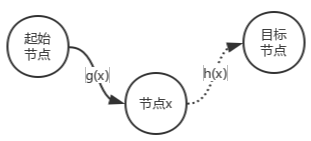
\includegraphics[width=0.4\textwidth]{informed.png}
    \caption{g(x)与h(x)示意图}
    \label{fig:informed}
    \end{figure}
    \item A*算法
    \begin{enumerate}[itemindent=1.5em,label=(\arabic*)]
      \item 算法描述
      \par \qquad A*算法是升级版的BFS算法,它每次边界节点中选出$f(x)$最小的节点扩展,计算邻节点的$g(x)$和$h(x)$值存入边界中。它维护两个列表,分别记为开启列表和关闭列表。开启列表存放边界节点,关闭列表存放所有已求出最优路径的节点。
      \par \qquad 一个节点$x$的相邻节点是那些可以通过交换空白块一步到达的状态。扩展$x$的相邻节点$n$时,需要将$g(n)$最小的$n$放入开启列表,因为$n$可以由几个节点扩展。一种做法是直接更新开启列表中$n$的$g(n)$值,另一种做法是在开启列表中保留$n$的多个副本,只访问第一次遇到的。
      \begin{figure}[H]
      \centering
      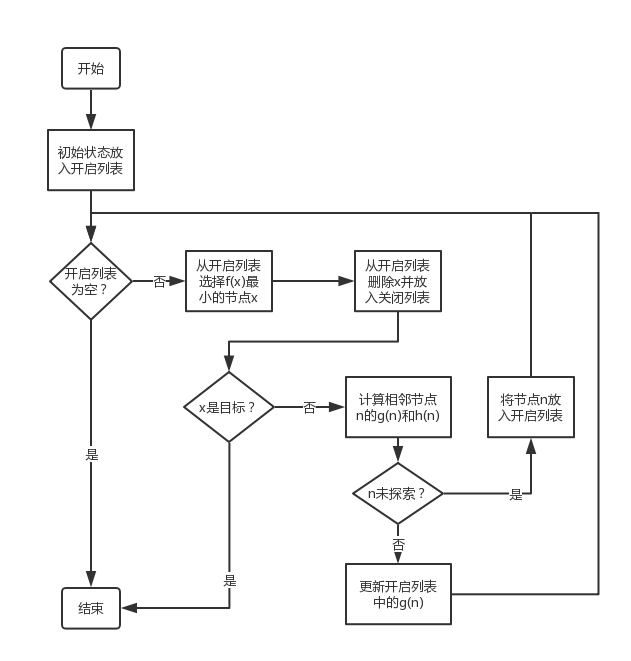
\includegraphics[width=0.8\textwidth]{astar.png}
      \caption{A*算法总体流程}
      \label{fig:astar}
      \end{figure}
      \item 优缺点
      \par \qquad 优点是时间复杂度与BFS相当;缺点是空间复杂度是指数级的,最坏情况下,在无界搜索空间中,扩展的节点数与解的深度$d$呈指数关系,为$O(b^d)$,其中$b$是后继节点的数目。
    \end{enumerate}

    \item IDA*算法
    \par \qquad 许多15 puzzle问题都无法通过A*算法来求解,因为它需要生成太多的新状态。假设用二维数组来表示拼图,那么每个新状态都是整个二维数组的拷贝,这无疑需要消耗很多内存来保存开启列表和关闭列表。
    \par \qquad IDA*(Iterative-Deepening-A*)克服了A*算法需要很大内存的缺点。它使用的是受限的DFS而不是BFS,在探索完一个节点后回溯,就能恢复拼图的状态,供下一个邻居使用,因此不需要拷贝二维数组。IDA*描述如下:
    \begin{enumerate}[itemindent=1.5em,label=(\arabic*)]
        \item 设置初始阈值为初始状态到目标状态的估计值;
        \item 执行一次DFS,对那些$f(x)$超过阈值的节点进行剪纸,即不再探索;
        \item 如果未找到解,增大阈值,回到步骤(2)。
    \end{enumerate}

    \begin{algorithm}
      \caption{IDA*的DFS算法}
        \begin{algorithmic}[1] %每行显示行号
          \Require $cur\_state$当前拼图状态,$cur\_cost$状态的实际代价,$threshold$迭代阈值,$Goal?$目标测试
          \Ensure 是否找到解,找到返回success, 找不到返回failure
            \Function {DFS}{$cur\_state, cur\_cost, threshold, Goal?$}
              \If {$cur\_cost + $h($cur\_state) > threshold$}
                \State \Return failure
              \EndIf
              \If {$Goal?(cur\_state)$}
                \State \Return success
              \EndIf
              \State $space\_i, space\_j \gets cur\_state$.space\_position()
              \For {$i,j \in$ successors($cur\_state$)}
                \State $cur\_state$.swap($i, j)$
                \If {DFS($cur\_state, cur\_cost + 1, threshold, Goal?$) == success}
                  \State \Return success
                \EndIf
                \State // 回溯
                \State $cur\_state$.swap($space\_i, space\_j$)
              \EndFor
              \State \Return failure
            \EndFunction
        \end{algorithmic}
    \end{algorithm}
    \item 启发函数的设计
    \par \qquad 启发函数最大的作用在于剪枝,它直接关系到需要探索的状态的多少。一个好的启发函数应该使所有节点的预计距离与真实距离接近,这样每次探索时基本都在选择最优路径上的节点。在实际应用中,15 puzzle问题主要有以下几种启发函数:
    \begin{enumerate}[itemindent=1.5em,label=(\arabic*)]
      \item \textbf{曼哈顿距离}:计算每个数码与目标位置的坐标各个维度的差的绝对值,即:
      \begin{equation}
        Manhattan(x,y) = \sum_{i=1}^d abs(x_i - y_i)
      \end{equation}
      其中d是坐标维度。
      \item \textbf{曼哈顿距离+线性冲突(linear conflict)}

      \begin{myDef}
        \textbf{线性冲突} 假设数码$t_j$和$t_k(t_j < t_k)$在同一行或同一列,并且它们的目标位置也在这一行或这一列。如果现在$t_j$在$t_k$的右边或下面,则它们是线性冲突的。
      \end{myDef}
      \par \qquad 曼哈顿距离忽略了一个事实——数码A要移动到数码B的位置,数码B就需要先移开。例如\figref{fig:lc-start}到\figref{fig:lc-goal}的曼哈顿距离是4,而实际上从\figref{fig:lc-start}到\figref{fig:lc-goal}需要经过至少6步,因为数码1要先往下移动,给数码3“腾出”位置。
      \begin{figure}[H]
      \centering
      \subfigure[起始]{
      \includegraphics[width=0.1\textwidth]{lc/start.png}
      \label{fig:lc-start}}
      \subfigure[第一步]{
      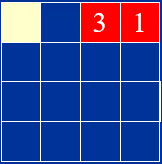
\includegraphics[width=0.1\textwidth]{lc/2.png}
      \label{fig:lc-1}}
      \subfigure[第二步]{
      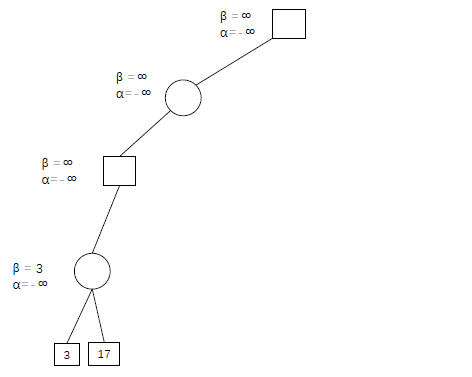
\includegraphics[width=0.1\textwidth]{lc/3.png}
      \label{fig:lc-2}}
      \subfigure[第三步]{
      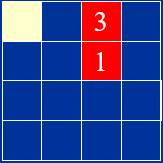
\includegraphics[width=0.1\textwidth]{lc/4.png}
      \label{fig:lc-3}}
      \subfigure[第四步]{
      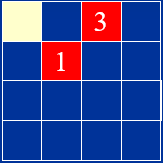
\includegraphics[width=0.1\textwidth]{lc/5.png}
      \label{fig:lc-4}}
      \subfigure[第五步]{
      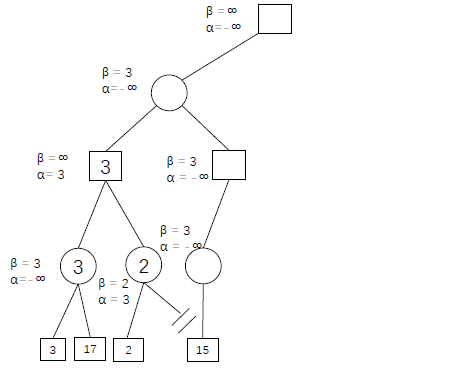
\includegraphics[width=0.1\textwidth]{lc/6.png}
      \label{fig:lc-5}}
      \subfigure[目标]{
      \includegraphics[width=0.1\textwidth]{lc/goal.png}
      \label{fig:lc-goal}}
      \end{figure}

      \par \qquad 要计算线性冲突距离,就需要{\color{red}统计拼图中有几对线性冲突的数码}。{\color{red}最终的距离是对数的2倍},因为每对线性冲突的数码,想要移动到目标位置,就需要其中一个先移动到其他行,等另一个移动完成后,它再移动回原来的行,这个过程至少需要额外的2步。
      \begin{algorithm}
        \caption{计算数码$x$线性冲突距离}
          \begin{algorithmic}[1] %每行显示行号
              \Require 拼图$puzzle$,$x$的当前坐标$(i,j)$,拼图大小$n$
              \Function {linear\_conflict}{$puzzle, i, j, n$}
                \State $x \gets puzzle[i][j]$
                \State $goal\_i,goal\_j \gets$ goal\_pos($x$)
                \State $count \gets 0$
                \State // 每个元素只检查它后面的元素
                \For {$k \in [j+1,n)$}
                  \State $y \gets puzzle[i][k]$
                  \State // x > y是产生冲突的前提,x-y<n表明可能在目标状态的同一行
                  \If {$y$ != $0$ \textbf{and} $x$ > $y$ \textbf{and} $x - y$ < $n$}
                    \State $y\_goal\_i,y\_goal\_j \gets$ goal\_pos($y$)
                    \If {$goal\_i == y\_goal\_i$}
                      \State $count \gets count + 1$
                    \EndIf
                  \EndIf
                \EndFor
                \State 同理,在列上重复以上循环
                \State \Return 2 * count
              \EndFunction
          \end{algorithmic}
      \end{algorithm}

    %   \item disjoint pattern database heuristic
    %   \par \qquad 该方法的基本思想是保存当前状态每个可能的子问题的实际代价,相加作为当前状态的估计代价。例如,对于\figref{fig:ap-start},将其分为红色和蓝色两个不重叠的子问题,移动红色到目标\figref{fig:ap-goal}需要20步,移动蓝色需要25步,那么启发函数返回就是45=20+25。该方法最特殊的情况就是Manhattan启发函数,将当前状态分为15个子问题,每个子问题含有一个数码。
    %   \begin{figure}[H]
    %   \centering
    %   \subfigure[起始]{
    %     \includegraphics[width=0.2\textwidth]{ap/start.png}
    %     \label{fig:ap-start}}
    %     \subfigure[目标]{
    %     \includegraphics[width=0.2\textwidth]{ap/goal.png}
    %     \label{fig:ap-goal}}
    %   \end{figure}
    \end{enumerate}
\end{enumerate}

\newpage
\zhsubsec {关键代码}
\begin{enumerate}[itemindent=2.5em,label=\arabic*、]
  \item 拼图压缩
  \par \qquad 正常情况下,如果使用整形二维数组存储拼图,假设每个整数的大小是4个字节,那么表示15 puzzle就需要$16 \times 4=64$个字节。然而,15 puzzle中的数字是0-15,使用4位(BITWISE)来表示一个数码就已经足够,这样总共需要8个字节,只有原来的$\frac{1}{8}$。如代码清单\ref{code:zip},使用64位无符号整形(uint\_fast64\_t)来表示拼图,位运算实现取数和存数操作。

\begin{lstlisting}[caption=拼图压缩,label={code:zip},captionpos=b]
// 1111,用于取低4位
#define LOWERBIT 15
class Puzzle {
  uint_fast64_t _puzzle;         // 16个数刚好用去64位
public:
  int space_i, space_j;    // 空白块的位置
  static const Puzzle goal(0x0FEDCBA987654321ULL);

  explicit Puzzle(uint_fast64_t puzzle = 0) : _puzzle(puzzle) { }
  // 实现类似于二维数组下标索引的get、set接口
  int get(int i, int j) const {
      // 计算偏移量,与位数相乘,得到(i,j)元素最低位的地址
      i = (i * 4 + j) * BITWISE;
      // 右移,取低4位就是(i,j)元素
      return (_puzzle >> i) & LOWERBIT;
  }
  void set(int i, int j, int x) {
      uint_fast64_t x64 = LOWERBIT;;
      int offset = (i * 4 + j) * BITWISE;
      _puzzle &= ~(x64 << offset);    // 先将(i,j)元素置为0
      x64 = x;
      _puzzle |= (x64 << offset);     // 左移取或就能把(i,j)置为x
      if (x == 0) {
          space_i = i;
          space_j = j;
      }
  }
  // 移动(i,j)位
  void swap(int i, int j) {
      set(space_i, space_j, get(i, j));
      set(i, j, 0);
  }
}
\end{lstlisting}

\item A*算法
\par \qquad 代码清单\ref{code:A*}维护了两个列表,一个是$open\_set$优先队列,相当于开启列表,它存储所有未找到最优路径的节点;另一个是{\color{red}$close\_set$哈希表,由于拼图是一个64位整数,哈希的键就是这个整数的哈希值,比康托展开快数倍}。在探索一个节点时,先用$can\_visit$函数检测节点是否在关闭列表或找到一个更短的最优路径,并将节点和当前的实际代价存入关闭列表$close\_set$;扩展节点时也用$can\_visit$检测从而把具有更小实际代价的邻居节点放入开启列表$open\_set$。
\par \qquad 理论上,第一次探索一个节点时,就找到了从起始节点到它的最优路径,因此探索节点时$can\_visit$检测似乎没必要。但是在实际运行程序时发现如果不检测就找不到最优路径。经过思考,认为是当状态空间存在环路,即一种拼图X可以从多种不同的拼图得来,这样当A*算法在非最优路径上探索到X时,会认为找到了最优路径,而实际上回溯再次探索到X时的花费可能更少。
\begin{lstlisting}[caption=A*,label={code:A*},captionpos=b]
void astar_search(const Puzzle& start, Heuristic* h, vector<int>& path) {
  ...
  auto* start_node = new node_type(start, h);
  open_set.push(start_node);      // open_set是一个极小堆,按f(x)排序
  while (!open_set.empty()) {
      node_type* node = open_set.top();   // 取出f(x)最小的一个节点
      open_set.pop();
      // 开启集合中可能有node的多个副本,访问最小的一个
      if (can_visit(close\_set, node->puzzle, node->cost)) {
          if (node->puzzle == node->puzzle.goal)
              break;
          close\_set[node->puzzle] = node->cost;
          // dy、dx组合成四个方向,返回空白块四个方向邻居的坐标
          node->puzzle.neighbors(dy, dx, neighbors);
          for (auto &neighbor : neighbors) {
              if (neighbor.first > -1 && neighbor.second > -1) {
                  // 生成一个新的相邻节点,并移动位数码
                  auto *n = new node_type(node,neighbor.first,neighbor.second);
                  if (can_visit(close\_set, n->puzzle, n->cost))
                      open_set.push(n);
              }
          }
      }
  }
  ...
}
\end{lstlisting}

\newpage
\item IDA*算法
\par \qquad 迭代加深的A*算法最关键的部分就是DFS。在每次递归,需要保证算法不会走回头路。也就是说,如果上一步交换空白块右边的块B,这样B就在空白块左边了,那么下一步就不应该交换左边的B。
\par \qquad 代码清单\ref{code:IDA*-DFS}使用了一个小技巧——如果当前方向$i$等于前一个方向$prev\_dir \oplus 1$,那么它们就是相反的方向。这是因为$dy$和$dx$方向数组被设计成上、下、左、右的顺序,容易验证$0 == 1 \oplus 1$、$1 == 0 \oplus 1$,2、3同理。
\par \qquad DFS的重中之重是回溯,交换了拼图$node$后,往下递归如果没有找到解,就需要换回来恢复原本的拼图,以供下一个邻居交换。
\begin{lstlisting}[caption=IDA*-DFS,label={code:IDA*-DFS},captionpos=b]
// prev_dir记录上一次移动的方向
bool dfs(Puzzle& node, int cost, int estimate,
        int limit, int prev_dir, Heuristic* h, vector<int>& path) {
    if (node == node.goal) return true;
    if (cost + estimate > limit) return false;

    int space_i = node.space_i, space_j = node.space_j;
    int exchange;
    pair<int, int> neighbors[4];

    node.neighbors(dy, dx, neighbors);    // 获取空白块四个方向邻居的坐标
    for (int i = 0; i < 4; i++) {
        if (i == (prev_dir ^ 1))    // 0上1下2左3右,不走回头
            continue;
        int ni = neighbors[i].first, nj = neighbors[i].second;
        if (ni > -1 && nj > -1) {
            exchange = node.get(ni, nj);
            // 从node移动(ni,nj)块变成相邻节点的相对距离
            int relative = h->relative_distance(node, ni, nj);
            path.push_back(exchange);
            // 更新g(x)和h(x)继续dfs,找到解则返回
            if (dfs(node, cost + 1, estimate + relative, limit, i, h, path))
                return true;
            // 找不到解需要回溯,恢复拼图,去掉白探索的路径
            path.pop_back();
            node.swap(space_i, space_j);
        }
    }
    return false;
}
\end{lstlisting}

\newpage
\item 线性冲突相对距离
\par \qquad 要计算相对距离,一个很自然的问题是,交换之后哪些数码被影响了?考虑\figref{fig:lc-node}到\figref{fig:lc-neighbor}的情况,现在想要交换数码3得到新的邻居节点。显然,0和3数码所在的位置必受影响。此外,由于计算一个数码的线性冲突个数需要遍历同一行、列后面的元素,因此数码0和3{\color{red}同一行、列前面的块}也受影响。如\figref{fig:lc-influence}红色的块。

\begin{figure}[H]%靠文字内容的左侧
\centering
\subfigure[node]{
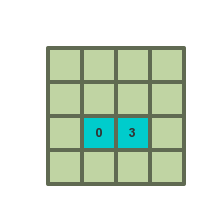
\includegraphics[width=0.2\textwidth]{lc-start.PNG}
\label{fig:lc-node}}
\subfigure[相邻节点]{
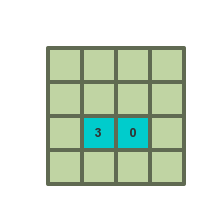
\includegraphics[width=0.2\textwidth]{lc-neighbor.PNG}
\label{fig:lc-neighbor}}
\subfigure[受影响的块]{
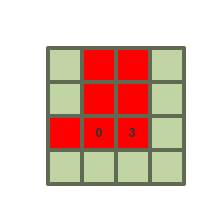
\includegraphics[width=0.2\textwidth]{lc-influence.PNG}
\label{fig:lc-influence}}
\end{figure}

\begin{lstlisting}[caption=线性冲突相对距离,label={code:lc-r},captionpos=b]
int lc_relative_distance(Puzzle& b, int i, int j) {
    int d = 0;
    if (i == space_i) {
        d -= linear_conflict(b, i, j);
        // 第j列、第space_j列在(i,j)块和空白块前的元素
        for (int k = 0; k < i; ++k)
            d -= linear_conflict(b, k, j) + linear_conflict(b, k, space_j);
        // 第i行在(i,j)块和空白块前的元素
        for (int k = 0; k < j && k < space_j; ++k)
            d -= linear_conflict(b, i, k);
        b.swap(i, j);
        d += linear_conflict(b, space_i, space_j);
        for (int k = 0; k < i; ++k)
            d += linear_conflict(b, k, j) + linear_conflict(b, k, space_j);
        for (int k = 0; k < j && k < space_j; ++k)
            d += linear_conflict(b, i, k);
    else {    // 列相同同理
      ...
    }
    return d;
}
\end{lstlisting}
\end{enumerate}

\newpage
\section{创新点\&优化}
\begin{enumerate}[itemindent=1.5em,label=\arabic*、]
  \item \textbf{优化拼图矩阵的拷贝}
  \par \qquad 对拼图矩阵进行压缩,用一个64位整数来表示整个拼图而不是$4 \times 4$整数矩阵;并且直接对这个整数哈希存入关闭列表,而且比康托展开快。
  \item \textbf{优化距离计算过程}
  \par \qquad 使用相对距离而不是绝对距离,即计算一次绝对距离,之后从一种状态到另一种状态的转换只需重新计算那些受影响的块,其他块的启发距离不变;
  \item \textbf{使用线性冲突(linear conflict)启发函数}
  \par \qquad Manhattan、Minkowski、Dijkstra三种启发函数都过小地估计了节点的距离(依次减小),通过在Manhattan距离上加上线性冲突,更接近真实距离。
\end{enumerate}
\section{实验结果及分析}
\par 实验中使用了两种算法(A*和IDA*)、两种关闭列表(字典和哈希表)、两种启发函数(Manhattan和Manhattan+Linear Conflict)、两种距离计算方式(相对和绝对)。表\ref{table:r-time}、\ref{table:a-time}分别列出了使用相对和绝对距离时算法的运行时间。
\par 首先,四个样例中样例2、4、1、3的求解时间依次递增,也就是说算法的运行时间和最优解的步数是正相关的。假设启发函数能使节点的估计代价接近真实代价,在A*算法中,这是因为BFS的探索过程会一层一层探索完那些估计代价小的节点,直至估计代价达到最优路径真实代价;在IDA*算法中,阈值的迭代也会达到最优路径的真实代价。
\par 其次,Manhattan+Linear Conflict启发函数比Manhattan启发函数更优。因为前者在后者的基础上增加了,而且是可采纳的,这样它的估计值就比后者更接近真实距离,进而减少了需要探索的状态空间的大小,即探索的过程更偏向于最优路径。
\par 再次,IDA*算法比A*算法更优。在时间复杂度上,IDA*与A*相当,这类似于迭代加深搜索和BFS。但是,IDA*最显著的优点是它不需要对状态进行拷贝,而A*算法每形成一个新状态都要拷贝整个拼图,这大大减少了IDA*算法的求解时间。
\par 另外,A*算法的关闭列表使用哈希表比使用字典更快(将近一半)。主要数据结构本身复杂度的问题,因为拼图已经做了压缩,字典是按拼图的字典序(实际上是64位整数的大小)存储,哈希表存储的是这个64位整数的哈希值,两者在数据拷贝方面相差无几。但是,使用拼图的哈希值存入关闭列表这种思想是很宝贵的,例如未对拼图压缩时,康托展开的哈希方法使关闭列表从矩阵的数组或字典变成哈希表,不仅省去拼图的拷贝过程,还大大减少拼图检索时间。
\par 最后,相对距离计算方法比绝对距离更优。这毋庸置疑,绝对距离每次都遍历整个拼图重新计算每个位置的距离,而相对距离只重新计算那些交换后受影响的位置,至少可以保证比遍历所有位置要少计算。

\begin{table}[H]
  \centering
  \caption{运行时间(/秒)——相对距离}
  \label{table:r-time}
  \begin{tabular}{c|c|c|c|c}
  \hline
  搜索策略 & 样例1 & 样例2 & 样例3 & 样例4\\
  \hline
  A*(Manhattan) & 650.09 & 15.95 & 969.81 & 46.43 \\
  A*(Manhattan+hashmap) & 304.53 & 8.47 & 411.39 & 22.04\\
  A*(Manhattan+linear conflict) & 160.85 & 2.29 & 207.85 & 14.4 \\
  A*(Manhattan+linear conflict+hashmap) & 84.52 & 1.72 & 99.96 & 8.21 \\
  IDA*(Manhattan) & 449.57 & 2.75 & 778.88 & 10.49 \\
  IDA*(Manhattan+linear conflict) & 81.75 & 3.04 & 304.83 & 9.55 \\
  \hline
  \hline
  \end{tabular}
\end{table}

\begin{table}[H]
  \centering
  \caption{运行时间(/秒)——绝对距离}
  \label{table:a-time}
  \begin{tabular}{c|c|c|c|c}
  \hline
  搜索策略 & 样例1 & 样例2 & 样例3 & 样例4\\
  \hline
  IDA*(Manhattan) & 1371.57 & 8.42 & 2362.81 & 31.91 \\
  IDA*(Manhattan+linear conflict) & 137.1 & 5.27 & 509.78 & 15.9 \\
  \hline
  \hline
  \end{tabular}
\end{table}

\section{思考题}
\zhsubsec{估价值和真实值的差距会造成算法性能差距的原因?}
\par 不妨假设两种算法需要探索的状态空间大小都是$b^d$,其中$d$是最优路径的深度。一个好的启发函数能对这$b^d$个节点起到很好的剪枝作用。对于A*算法来说,它贪婪地选择探索估计代价最小的节点,如果估计值接近真实值,那么算法每次都能选择最优路径上的节点来探索,直到找到目标节点后返回,这样就只探索了$d$个节点;对于IDA*算法来说,如果估计值接近真实值,阈值的迭代次数就会少很多(极端情况下估计值等于真实值时,只需迭代一次就能找到解)。
\end{document}
